% !TEX root = ../YourName-Dissertation.tex

\chapter{Neutrinos and Neutrino Masses}

\section{Introduction}

In this chapter I provide a cursory overview of background information relevant to neutrinos and neutrino mass measurements. 

In Section \ref{sec:chap2-nu-history} I provide background information on the history of neutrinos and beta-decay. In Section \ref{sec:chap2-nu-oscillation} I describe the discovery of neutrino oscillations, which demonstrated unambiguously that neutrinos have non-zero masses. In Section \ref{sec:chap2-nu-mass-sm} I discuss the current state of the theoretical understanding of neutrino masses in the standard model. Lastly, in Section \ref{sec:chap2-nu-mass-scale} I discuss a few methods for measuring the absolute scale of the neutrino mass.

\section{Neutrinos and Beta-decay}
\label{sec:chap2-nu-history}
Late in the 19th century the phenomena of radioactivity was first observed in experiments performed by Henri Becquerel with uranium, and further studied using thorium and radium by Marie and Pierre Currie \cite{nuclear_physics, curie}. Early work in radioactivity classified different forms of radiation based on it's ability to penetrate different materials. Rutherford was the first to separate radioactive emissions into two types, alpha and beta radiation \cite{rutherford_rad_types}. Alpha rays were easily stopped by a piece of paper or thin foil of metal, whereas beta radiation could penetrate metal several millimeters thick. Later a third form of radiation was identified by Villard \cite{villard}, which was still more penetrating, later termed gamma radiation by Rutherford. 

When these forms of radioactivity were first discovered, it was unclear what physically constituted an alpha, beta, or gamma particle. Experiments with radioactivity in magnetic fields ware eventually able to identify the charge composition of the different forms of radiation. In particular, experiments by Becquerel identified \cite{Becquerel_beta_electron} that beta radiation had an identical charge-to-mass ratio to the electron. This was strongly suggestive that beta particles were indeed electrons.

Studies of beta radiation lead to the discovery that radioactivity resulted in the transmutation of elements \cite{rutherford_transmutation} caused by the decay of a heavier nucleus to a lighter species. A decay that produces beta-radiation is called a beta-decay. One feature of beta radiation that differentiated it from alpha and gamma radiation is that the electrons produced by beta-decay have a continuous spectrum of kinetic energies, whereas, alpha and gamma particles are emitted with discrete energies. This feature of beta-decay was first observed by Chadwick in 1914 \cite{chadwick1914}, and was extremely puzzling at the time, since the continuous spectrum apparently violates energy conservation \cite{bohr_energy_nonconservation_ref}. 

Famously, in 1930 Pauli proposed the existence of a new neutral particle, which he termed the "neutron", that was also produced during beta-decay to resolve the missing energy problem posed by the beta-decay spectrum \cite{Pauli:1930pc}. Because this particle carried no charge, it was hypothesized that it had simply not been observed in any previous experiments. This "neutron", which was initially estimated to have a mass no larger than that of an electron, was eventually renamed the "neutrino" by Fermi \cite{fermi_rename} after the discovery of the neutron by Chadwick in 1932 \cite{neutron}. Later, in 1933, Fermi developed a quantum mechanical theory for beta-decay in which an electron and neutrino are produced by the decay of a neutron to a proton inside the radioactive nucleus \cite{fermi_beta_decay}.

Little more than a speculation when first introduced, indirect evidence for the existence of neutrinos was obtained in 1938 by the simultaneous observation of the electron and recoiling nucleus in cloud chambers by Crane and Halpern \cite{crane_halpern}. However, it wasn't until the Cowan-Reines experiment \cite{cowan_reines} in 1956 that direct evidence for the existence of neutrinos was observed through the observation of inverse beta-decays caused by neutrinos from a nuclear reactor interacting with protons contained in water molecules. The difficulty in detecting neutrinos is caused by their weak interactions with other particles. Later experiments revealed the existence of different types or flavors of neutrinos based on the nature of the leptons produced in neutrino charged-current interactions \cite{neutrino_flavor}, but the existence of a neutrino mass remained an open question that would take more than 40 year to resolve.

\section{Neutrino Oscillations}
\label{sec:chap2-nu-oscillation}

One of the first clues that neutrino flavor transitions or neutrino oscillations were occurring was the solar neutrino problem. The solar neutrino problem is a discrepancy between the measured and predicted flux of $\nu_e$ from the sum. The solar neutrino problem was famously observed by Ray Davis Jr. and collaborators in the 1960's \cite{ray_davis} at the Homestake mine in South Dakota. In the early 2000's, the SNO experiment was able to resolve the solar neutrino problem by identifying neutrino oscillations as the cause of the observed deficit \cite{SNO}. Furthermore, measurements of the atmospheric flux of neutrinos by the Super-Kamiokande experiment and others revealed that fewer muon-type neutrinos survived passage through the earth than expected providing strong evidence for neutrino oscillations for both flavors \cite{superk}.

Neutrino oscillations occur because the neutrino flavor eigenstates are distinct from the mass eigenstates \cite{nu_oscillations}. The neutrino mass eigenstates represent physical particles in that they are solutions to the free-particle Hamiltonian, whereas, the neutrino flavor eigenstates correspond to the neutrino states that interact via the weak charged-current interaction. The neutrino flavor eigenstates are a linear superposition of the neutrino mass eigenstates
\begin{equation}
    \nu_\ell=\sum_i{U_{\ell i}\nu_i},
\end{equation}
where $\ell=e,\mu,\tau$ and $i=1,2,3$. The matrix elements $U_{\ell i}$ are the elements of the Pontecorvo-Maki-Nakagawa-Sakata (PMNS) matrix that describes the mixing between the neutrino flavor and mass states.

\begin{figure}[htbp]
    \centering
    \includegraphics[width=0.5\textwidth]{figs/Chapter-2/230227_chap2_nu_hierarchy.png}
    \caption{A diagram of two different neutrino mass ordering scenarios \cite{nu_mass_ordering_figure_inspiration}. In the inverted hierarchy (inverted mass ordering) the lightest neutrino mass is $m_3$, whereas,in the normal hierarchy (normal mass ordering) $m_1$ is the lightest neutrino. What cannot be measured by neutrino oscillations is the neutrino absolute mass scale, which is essentially the mass of the lightest neutrino mass eigenstate.}
    \label{fig:chap2-nu-hierarchy}
\end{figure}

A standard parameterization \cite{Workman:2022ynf} of the PMNS matrix is 
\begin{equation}
    \begin{split}
        U_{PMNS}=&\begin{bmatrix}
            U_{e1}&U_{e2}&U_{e3}\\
            U_{\mu 1}&U_{\mu 2}&U_{\mu 3}\\
            U_{\tau 1}&U_{\tau 2}&U_{\tau 3}
        \end{bmatrix}\\
        =&\begin{bmatrix}
            1&0&0\\0&c_{23}&s_{23}\\0&-s_{23}&c_{23}
        \end{bmatrix}
        \begin{bmatrix}
            c_{13}&0&s_{13}e^{-i\delta}\\0&1&0\\-s_{13}e^{i\delta}&0&c_{13}
        \end{bmatrix}
        \begin{bmatrix}
            c_{12}&s_{12}&0\\-s_{12}&c_{12}&0\\0&0&1
        \end{bmatrix}\\
        &\times
        \begin{bmatrix}
            e^{i\alpha_1/2}&0&0\\
            0&e^{i\alpha_2/2}&0\\
            0&0&1
        \end{bmatrix},
    \end{split}
\end{equation}
where $c_{ij}=\cos{\theta_{ij}}$ and $s_{ij}=\sin{\theta_{ij}}$. The parameters $\alpha_1$ and $\alpha_2$ are only included in the PNMS matrix if neutrinos are Majorana particles, something which represents a current area of research in neutrino physics. The phase $\delta$ quantifies the degree of CP-violation in the neutrino sector. Including the Majorana phases the PMNS matrix contains six independent parameters. Neutrino oscillation probabilities also depend on the squared mass differences between neutrino mass eigenstates
\begin{equation}
    \Delta m_{ij}^2=m_i^2-m_j^2,
\end{equation}
where $ij=12,32,31$ respectively. Because $\Delta m_{32}^2=\Delta m_{31}^2-\Delta m_{21}^2$, this adds an additional two parameters that must be constrained by neutrino oscillations. 

A large experimental effort over the past couple decades has greatly contained the majority of parameters in the PMNS matrix, many to relative uncertainties of only a few percent. However, certain ambiguities remain, which is the origin of the current uncertainty in the ordering of the neutrino masses (see Figure \ref{fig:chap2-nu-hierarchy}). The neutrino masses can be arranged by their relative masses. Current neutrino oscillation data supports that $m_2>m_1$, however, the sign of $\Delta m_{32}^2$ is still unknown. Therefore, two mass-ordering scenarios are allowed, one where neutrino masses are arranged $m_3>m_2>m_1$, which is called the normal mass ordering (NMO), or alternatively neutrino masses may be ordered $m_2>m_1>m_3$, which is called the inverted mass ordering (IMO). Next-generation neutrino oscillation experiments such as JUNO \cite{JUNO}, Hyper-Kamiokande \cite{hyperk}, and DUNE \cite{DUNE} are poised to resolve this ambiguity in the coming years.

Neutrino oscillation probabilities are sensitive to the neutrino masses via the squared mass differences. Therefore, oscillation probabilities are unaffected by the absolute scale of the neutrino mass. However, oscillations can be used to obtain a lower bound on the neutrino masses by setting the mass of the lightest neutrino mass state to zero. This results in different lower limits depending on the ordering of the neutrino mass states. Current best-fit values \cite{Workman:2022ynf} with $1\sigma$-uncertainties for the squared mass differences are 
\begin{align}
    \Delta m_{21}^2&=(7.42^{+0.21}_{-0.20})\times 10^{-5}\text{ eV}^2,\\
    \Delta m_{31}^2&=(2.5176{+0.026}_{-0.028})\times 10^{-3}\text{ eV}^2\text{ (NMO)},
\end{align}
for the normal mass ordering, and for the inverted ordering the limit is
\begin{align}
    \Delta m_{32}^2&=(-2.498^{+0.028}_{-0.028})\times 10^{-3}\text{ eV}^2\text{ (IMO)}.
\end{align}
The parameter $\Delta m_{21}^2$ is the same in the NMO and the IMO. Allowing the lightest neutrino mass in each ordering scenario ($m_\textrm{least}$) to take on a range of values, one can visualize the relative masses of the neutrinos as a function of $m_\textrm{least}$ (see Figure \ref{fig:chap2-mass-estates}). The absolute neutrino mass scale is effectively the value of this $m_\textrm{least}$ parameter.

\begin{figure}[htbp]
    \centering
    \begin{subfigure}{0.49\textwidth}
        \includegraphics*[width=\textwidth]{figs/Chapter-2/230302_mass_estate_vals_normal.png}
        \caption{}
    \end{subfigure}
    \hfill
    \begin{subfigure}{0.49\textwidth}
        \includegraphics*[width=\textwidth]{figs/Chapter-2/230302_mass_estate_vals_inverted.png}
        \caption{}
    \end{subfigure}
    \caption{The masses of the neutrinos as a function of the lightest neutrino mass in both the normal (a) and inverted (b) mass ordering regimes.}
    \label{fig:chap2-mass-estates}
\end{figure}

%Various extensions to the 3x3 mixing regime, so called sterile neutrinos, have been proposed to explain certain anomalous neutrino oscillation phenomena observed primarily in neutrinos produced by nuclear reactors. Currently there is inconclusive evidence to support the existence of sterile neutrinos. Certain of these apparently anomalous results can be explained by better modeling of the nuclear processes in the reactors that generate the measured flux of neutrinos. However, some puzzles such as the unexplained neutrino deficits measured by the BEST experiment remain open.  

\section{Neutrino Masses in the Standard Model}
\label{sec:chap2-nu-mass-sm}

In this section, I briefly summarize the current theoretical understanding of neutrino masses in the standard model \cite{nu_physics1, nu_physics2, nu_physics3}. Neutrinos are spin 1/2 particles, which are described using the Dirac equation. 
\begin{equation}
    (i\hbar\gamma^\mu\partial_\mu-mc)\psi(x)=0, 
\end{equation}
where the field that describes the particle is denoted as $\psi(x)$. In the standard model fermions acquire mass through the Yukawa interaction, which add to the standard model Lagrangian terms of the form 
\begin{equation}
    \mathcal{L}_\textrm{Yukawa}=-Y^\ell_{ij}\bar{L}_{Li}\phi E_{Rj}+\textrm{h.c.},
\end{equation}
where $Y_{ij}^\ell$ is an element of the $3\times3$ Yukawa coupling matrix for leptons, $L_{Li}$ is the left-handed lepton doublet for generation $i$, $\phi$ is the Higgs doublet, and $E_{Rj}$ is the right-handed lepton field for generation $j$. Neutrinos are represented only as left-handed neutrinos and right-handed antineutrinos in the standard model, which is consistent with experimental observations. Since there are no right-handed neutrino singlet fields, there are no Yukawa interaction terms, thus neutrinos in the standard model are strictly massless. Therefore, non-zero neutrino mass is evidence for physics beyond the standard model. 

For the charged leptons, the Yukawa interaction leads to masses of the form 
\begin{equation}
    m^\ell_{ij}=Y^\ell_{ij}\frac{v}{\sqrt{2}},
\end{equation}
where $v$ is the Higgs vacuum expectation value. The observation of massive neutrinos motivates the extension of the standard model to explain the origin of neutrino masses, which can be approached in different ways, but all approaches add additional degrees of freedom to the standard model. 

One approach is to introduce to the standard model a right-handed neutrino field that allows one to include Yukawa terms of the form 
\begin{equation}
    \mathcal{L}_{\nu\textrm{Yukawa}} = -Y^\ell_{ij}\bar{L}_{Li}\phi \nu_{Rj}+\textrm{h.c.}
\end{equation}
where $\nu_{Rj}$ is the right-handed neutrino singlet. Because experimental evidence strongly predicts only three active neutrinos, these additional neutrinos are "sterile", in that they do not interact via the strong, weak, or electromagnetic interactions. After spontaneous symmetry breaking, the Yukawa interaction leads to mass terms given by 
\begin{equation}
    \mathcal{L}_{D}=-M_{Dij}\bar{\nu}_{Ri}\nu_{Lj} +\textrm{h.c.},
\end{equation}
which is called a Dirac mass term. One of the issues with constructing neutrino masses in this way is that the required Yukawa couplings are at least a factor of $10^6$ smaller than that of an electron, which begs the question: why are the Yukawa couplings so small for the neutrinos?

An alternative approach is to allow the neutrinos to have a Majorana mass, which is possible because neutrinos are electrically neutral particles. The Majorana mass terms for neutrinos have the form 
\begin{equation}
    \mathcal{L}_{M}=-\frac{1}{2}(M_{Rij}\bar{\nu}_{Ri}\nu_{Rj}^c M_{Lij}\bar{\nu}_{Li}\nu_{Lj}^c) +\textrm{h.c.},
\end{equation}
where $M_{Rij}$ and $M_{Lij}$ are right-handed and left-handed Majorana mass matrices. A consequence of neutrinos being Majorana particles is lepton number violation, which predicts the occurrence of neutrino-less double beta-decay at a rate proportional to the neutrino mass.

In the most general case neutrinos have both Dirac and Majorana mass terms, which allows one to generate neutrino masses with Yukawa couplings similar to the rest of the standard model. Considering a single generation of neutrinos for demonstration, the combined neutrino mass Lagrangian can be written as 
\begin{equation}
    \mathcal{L}_{D+M}=-m_D\bar{\nu}_{R}\nu_{L} - \frac{1}{2}(m_L\bar{\nu}_L\nu_L^c+m_R\bar{\nu}_R\nu_R^c)+\text{h.c.},
\end{equation}
or equivalently,
\begin{equation}
    \label{eq:chap2-see-saw-lagrangian}
    \mathcal{L}_{D+M}=-\frac{1}{2}\begin{bmatrix}\bar{\nu}_L&\bar{\nu}^c_R\end{bmatrix}\begin{bmatrix}m_L&m_D\\m_D&m_R\end{bmatrix}\begin{bmatrix}\nu^c_L\\ \nu_R\end{bmatrix} + \text{h.c.}.
\end{equation}
An example mass generation mechanism with this approach is the Type-I see-saw mechanism \cite{numass_models_seesaw}, in which one takes $m_L=0$ and $m_R\gg m_D$. By diagonalizing Equation \ref{eq:chap2-see-saw-lagrangian} one obtains the mass eigenvalues that represent the physical masses of the neutrinos. The light neutrino mass eigenstate, which represents the observed neutrino mass, has a mass given by
\begin{equation}
    m_1\approx\frac{m_D^2}{m_R},
\end{equation}
and the heavy neutrino mass eigenstate, which represents the unobserved sterile neutrino, has a mass
\begin{equation}
    m_2\approx m_R.
\end{equation}
For $m_D$ similar to the other quark or lepton masses, one obtains physical neutrino masses consistent with observations from sterile neutrino masses of $m_R\approx O(10^{15})$~GeV. This mass scale is well beyond the capabilities of modern particle accelerators to probe. 

\section{Neutrino Absolute Mass Scale}
\label{sec:chap2-nu-mass-scale}

The neutrino absolute mass scale or simply "neutrino mass" cannot be probed with neutrino oscillations, since oscillation probabilities are determined by the squared mass differences between neutrino mass eigenstates, therefore, alternative techniques are needed to perform an effective measurement of the neutrino mass.

\subsection{Limits from Cosmology}


The $\Lambda$CDM model summarizes the current cosmological understanding of the universe \cite{Workman:2022ynf}. $\Lambda$CDM predicts that the universe originated from a single expansion event colloquially called the "Big Bang". During the Big Bang, the universe originated as a hot spacetime singularity, which abruptly experienced rapid expansion in a process known as inflation. After expansion the inflationary field eventually decayed into a population of quarks, gluons, leptons, and photons, which were kept in thermal equilibrium by the high-temperatures of the early universe.

As the universe continued to expand it's density and temperature decreased until the formation of neutral atoms, primarily hydrogen, was possible. At which point the population of photons produced during the Big Bang decoupled from the primordial universe and began to freely propagate. A direct prediction of the $\Lambda$CDM model is that this population of photons is still present, but with a significantly reduced temperature due to the subsequent expansion of the universe. This is consistent with the observation of the CMB (cosmic microwave background), which is a population of microwave radiation with a blackbody temperature of 2.7~K. The CMB is extremely uniform in all directions with slight anisotropies that can be analyzed to study the evolution of the early universe. A series of experiments have measured the CMB with increasing levels of precision, which has lead to a significant increase in our current understanding of cosmology.

In addition to the CMB, inflation predicts the existence of a C$\nu$B (cosmic neutrino background) \cite{numass_cosmo}, which are the remnant neutrinos produced during the Big Bang. Since neutrinos only interact via the weak force, they decouple from the Big Bang plasma at an earlier time than the CMB photons. The temperature at which the C$\nu$B decouples depends on the neutrino rest mass. Neutrinos play a unique role in the $\Lambda$CDM model, due to the fact that neutrinos act as radiation early in the universe but as matter in the late universe. This leads to specific signatures that impact the expected anisotropies of the CMB as well as the distribution of matter in the universe \cite{planck2015}. By combining measurements of the CMB with measurements of the large-scale structure (LSS) of the universe one can constrain the neutrino mass scale by fitting these datasets with the $\Lambda$CDM model. This analysis results in some of the most stringent constraints on the neutrino mass. Recent analyses \cite{Workman:2022ynf} have been able to constrain the neutrino mass scale to
\begin{equation}
     \Sigma_{m_\nu} \equiv \sum_{i}m_i<0.11~\mathrm{eV},
\end{equation}
where $m_i$ are the neutrino mass eigenstates. 

\begin{figure}[htbp]
    \centering
    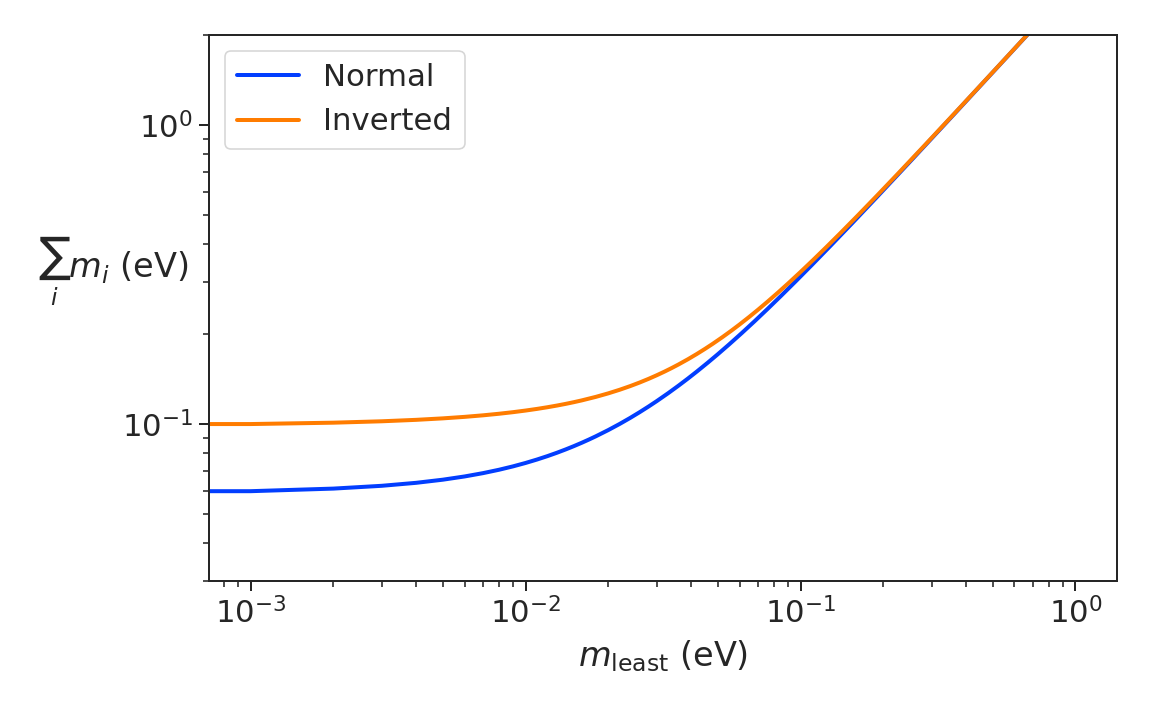
\includegraphics[width=0.6\textwidth]{figs/Chapter-2/230301_cosmology_nu_mass_observable.png}
    \caption{The neutrino mass observable measured by cosmology as a function of the lightest neutrino mass eigenstate.}
    \label{fig:chap2-nu-mass-cosmo}
\end{figure}

The observable $\Sigma_{m_\nu}$ constrains the neutrino mass by setting the mass of the lightest neutrino mass eigenstate ($m_\mathrm{least}$) (see Figure \ref{fig:chap2-nu-mass-cosmo}). In the normal mass ordering $\Sigma_{m_\nu}$ can be rewritten in the form 
\begin{equation}
    \Sigma_{m_\nu} = m_\mathrm{least} + \sqrt{\Delta m_{21}^2+m_\mathrm{least}^2}+\sqrt{\Delta m_{32}^2+m_\mathrm{least}^2},
\end{equation}
where it is clear that a measurement of $\Sigma_{m_\nu}$ effectively sets the neutrino mass scale through $m_\mathrm{least}$. The analogous formula for the inverted mass ordering is 
\begin{equation}
    \Sigma_{m_\nu} = m_\mathrm{least}+\sqrt{-\Delta m_{32}^2+m_\mathrm{least}^2}+\sqrt{-\Delta m_{31}^2+m_\mathrm{least}^2}.
\end{equation}

Upcoming experiments \cite{cmb_s4} are planned to refine measurements of the CMB, LSS, and other cosmological observables. With this additional data it is possible that in the near future cosmological measurements will be able to positively constrain the neutrino absolute mass scale. However, the strength of these limits strictly depend on the accuracy of the $\Lambda$CDM model, which highlights the need for direct experimental measurements of the neutrino mass to confirm the predictions of cosmology and to fix the neutrino mass parameter in future cosmological analyses.

\subsection{Limits from Neutrinoless Double Beta-decay Searches}

If neutrinos are Majorana fermions, then the neutrino is equivalent to its own antiparticle and lepton conservation is not an exact law of nature \cite{double_beta1}. Limits on the rate of neutrinoless double beta-decay ($0\nu\beta\beta$), are some of the most powerful current tests of lepton number conservation \cite{Workman:2022ynf}. If $0\nu\beta\beta$ were observed, it would be direct evidence that neutrinos are Majorana fermions and provide a method for measuring the neutrino mass scale.

Standard double beta-decay occurs when two neutrons in an unstable nucleus spontaneously decay into two protons, which results in the production of two electrons and two neutrinos (see Figure \ref{fig:chap2-0nubetabeta-diagram}).  
\begin{figure}[htbp]
    \centering
    \begin{subfigure}{0.4\textwidth}
        \includegraphics*[width=\textwidth]{figs/Chapter-2/230717_2nubetabeta.png}
        \caption{}
    \end{subfigure}
    \begin{subfigure}{0.4\textwidth}
        \includegraphics*[width=\textwidth]{figs/Chapter-2/230717_0nubetabeta.png}
        \caption{}
    \end{subfigure}
    \caption{\label{fig:chap2-0nubetabeta-diagram} Feynman diagrams for double beta-decay (a) and $0\nu\beta\beta$(b).}
\end{figure}
Whereas, during $0\nu\beta\beta$ the two neutrinos self-annihilate producing only two electrons, which violates lepton number by two. 

Assuming that the exchange of two Majorana neutrinos is the dominant channel for $0\nu\beta\beta$, then a measurement of the $0\nu\beta\beta$ half-life for a particular isotope can be used to set the neutrino absolute mass scale \cite{double_beta2}. The half-life is written in terms of the effective neutrino mass for $0\nu\beta\beta$ ($m_{\beta\beta}$) using the equation 
\begin{equation}
    T^{0\nu}_{1/2}=\frac{1}{G|\mathcal{M}|^2m_{\beta\beta}^2},
\end{equation}
where $G$ is the phase-space factor for the decay and $\mathcal{M}$ is the relevant nuclear matrix element. $m_{\beta\beta}$ is given by an incoherent sum of the neutrino mass eigenstates weighted by the PMNS mixing matrix parameters,
\begin{equation}
    m_{\beta\beta}=\left|\sum_{i}U_{ei}^2m_i\right|.
    \label{eq:chap2-mbetabeta}
\end{equation}

The information provided from $0\nu\beta\beta$ on the neutrino mass scale can be visualized by expressing the value of $m_{\beta\beta}$ in terms of $m_\textrm{least}$ and two relative Majorana phases \cite{double_beta_plot}. The allowed regions for $m_{\beta\beta}$ as a function of $m_\textrm{least}$ are shown in Figure \ref{fig:chap2-nu-mass-0nbb-posterior} as the regions bounded by the black curves overlayed with the discovery probabilities of future $0\nu\beta\beta$ decay experiments based on current neutrino data.
\begin{figure}[htbp]
    \centering
    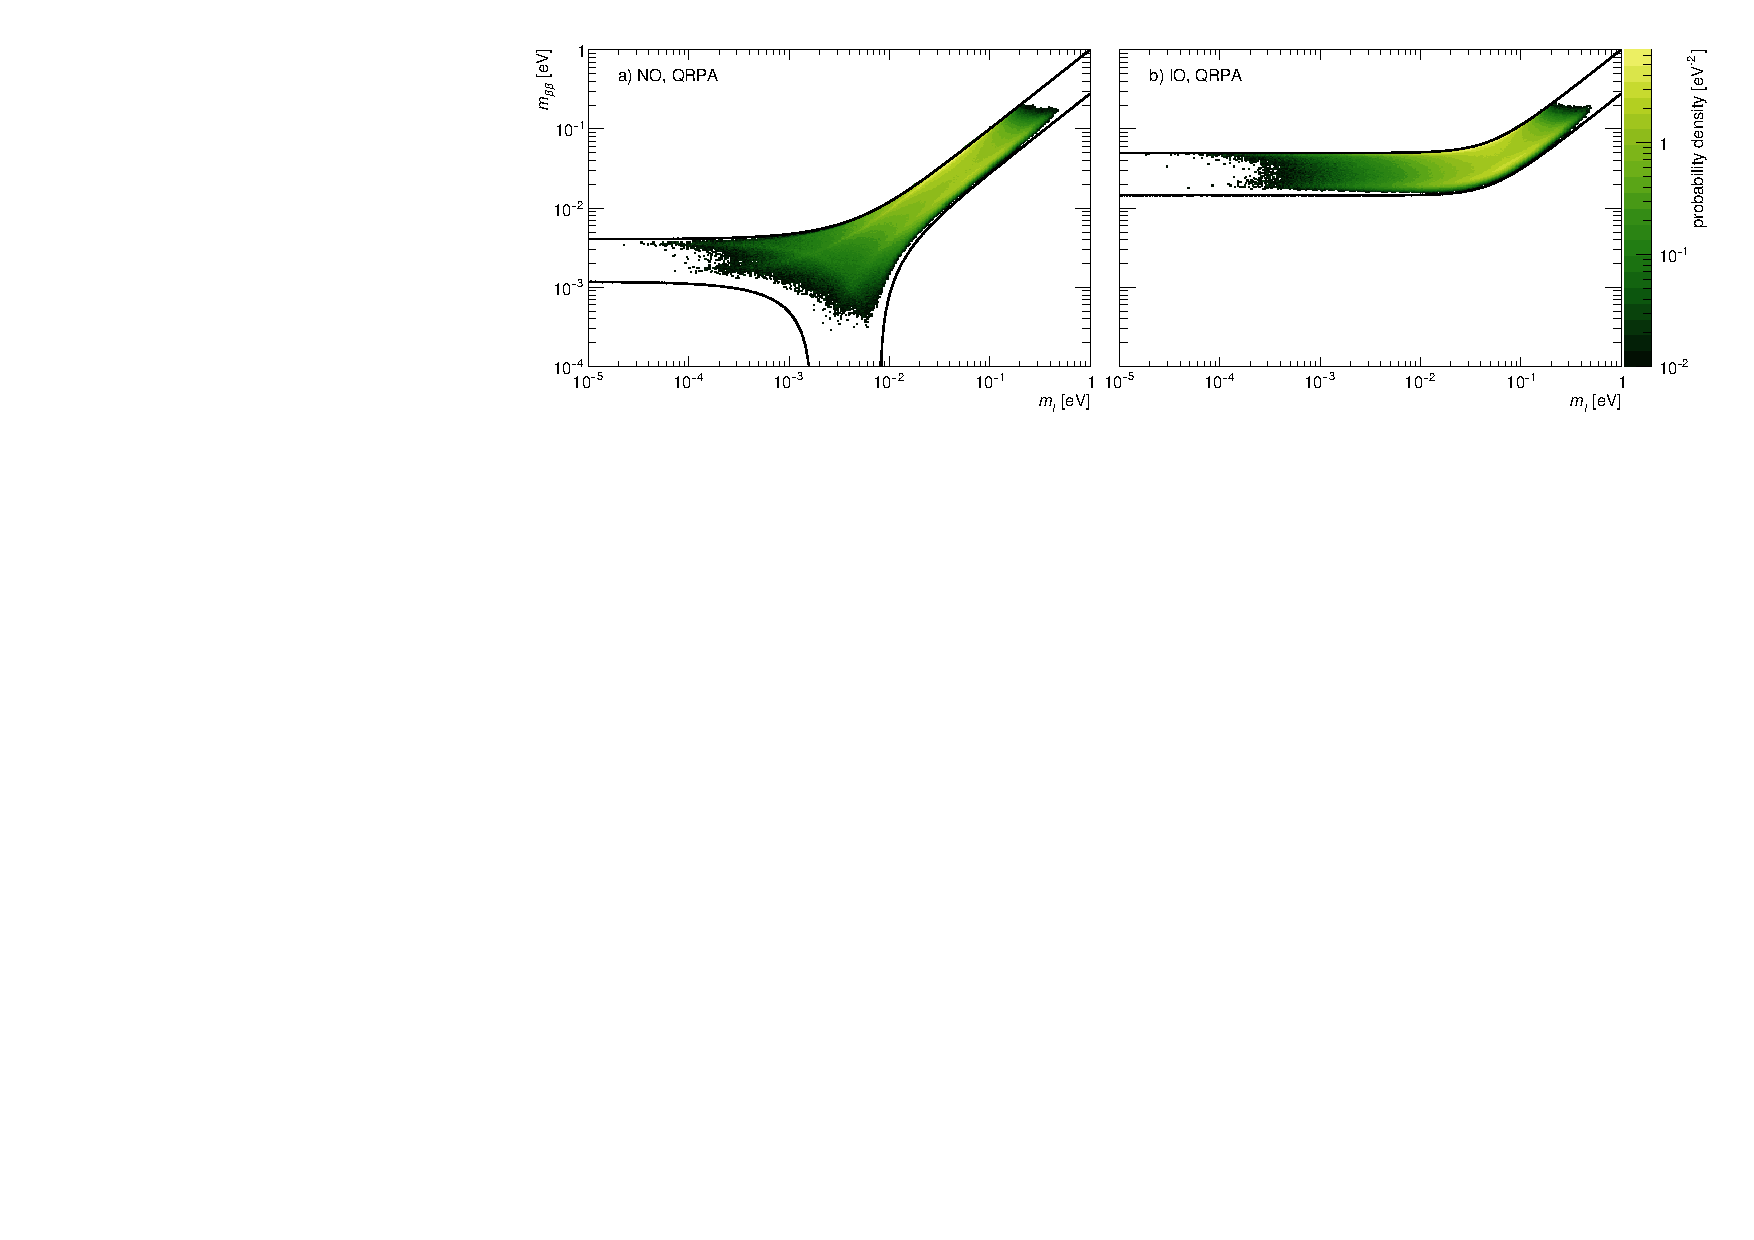
\includegraphics[width=1.0\textwidth]{figs/Chapter-2/230228_nu_mass_0nbb.pdf}
    \caption{The discovery probabilities for the future generation of $0\nu\beta\beta$ experiments as a function of $m_{\beta\beta}$ and $m_{least}$. Figure from \cite{double_beta_plot}.}
    \label{fig:chap2-nu-mass-0nbb-posterior}
\end{figure}

Because of the possibility of cancellation due to the unknown Majorana phases included in the sum specified by Equation \ref{eq:chap2-mbetabeta}, the neutrino mass information gained from $0\nu\beta\beta$ is necessarily imperfect. Additionally, theoretical uncertainties in the calculation of the nuclear matrix elements complicates the calculation of $m_{\beta\beta}$ from a measurement of $0\nu\beta\beta$ half-life. Similar to cosmology, there is a high degree of complementarity between direct measurements of the neutrino mass and $0\nu\beta\beta$. In particular, a measurement of $m_\textrm{least}$ to less than 0.1~eV sensitivity provides significant information for $0\nu\beta\beta$ searches based on the discovery probabilities displayed in Figure \ref{fig:chap2-nu-mass-0nbb-posterior}.

\subsection{Limits from Beta-decay}

\begin{figure}[htbp]
    \centering
    \includegraphics*[width=0.6\textwidth]{figs/Chapter-2/230717_betadecay.png}
    \caption{\label{fig:chap2-beta-decay-diagram} A Feynman diagram of beta decay}
\end{figure}

Certain processes involving neutrinos, in particular beta-decay (see Figure \ref{fig:chap2-beta-decay-diagram}), have initial states with well-defined total energies and final states that can be measured with high accuracy and precision. Beta-decay involves the decay of an unstable isotope where a neutron spontaneously converts to a proton and emits and electron and anti-neutrino ("neutrino" for brevity) to conserve charge and lepton number \cite{nuclear_physics}. Therefore, by applying the principles of energy and momentum conservation, a measurement of the kinematics of the final state can be used to constrain the neutrino mass \cite{FORMAGGIO20211}. 

Using beta-decay to measure the neutrino mass can be tied back to Fermi's original 1934 theory of nuclear beta-decay \cite{fermi_beta_decay} (see Figure \ref{fig:chap2-fermi-original-b-spectrum}).
\begin{figure}[htbp]
    \centering
    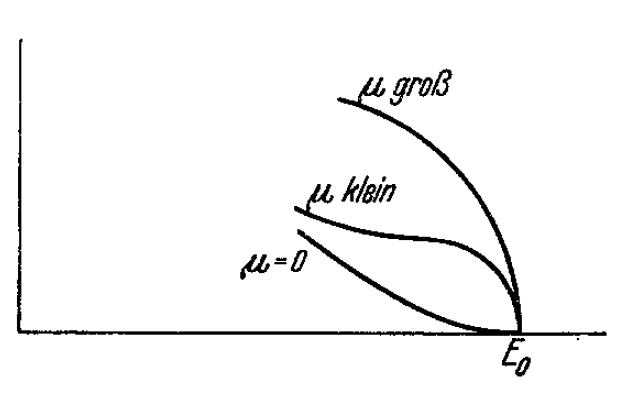
\includegraphics[width=0.5\textwidth]{figs/Chapter-2/Fermi.png}
    \caption{A figure from Fermi's 1934 paper on a theory of beta-decay depicting the kinetic energy spectrum of the emitted electron. The effect of the neutrino mass, written as $\mu$, is to distort the shape of the spectrum near the endpoint from the zero-mass spectrum.}
    \label{fig:chap2-fermi-original-b-spectrum}
\end{figure}
Because the constraints on the neutrino mass from beta-decay depend only on the final state measurement capabilities and the principles of energy and momentum conservation, neutrino mass measurements with beta-decay are called direct measurements. A direct measurement like beta-decay contrasts with other neutrino mass measurements approaches that are model-dependent such as cosmology and $0\nu\beta\beta$, which provide complementary ways to study the physics of massive neutrinos.

The isotope of choice for direct neutrino mass measurements with beta-decay has been tritium ($^3H_2$) for many decades, because it conveniently fulfills many experimental requirements. Of upmost importance is a decay with a low Q-value, which is the available kinetic energy based on the mass difference between the initial and final states. The effect of a massive neutrino on the shape of the spectrum is magnified for low Q-values and tritium has an unusually low Q-value of 18.6~keV.

Additionally, tritium beta-decay is super-allowed, which results in a relatively short half-life of 12.3~years. Therefore, high source activity can be obtained with a relatively small source mass. High-activity is desirable because of the low-activity near the tritium spectrum endpoint. For tritium beta-decays, only a factor of $3\times10^{-13}$ of the decays occur in the last 1~eV of the spectrum. Isotopes with Q-values lower than tritium are known \cite{FORMAGGIO20211}, but this is outweighed by exceedingly long half-lives leading to unobtainable source masses.

The endpoint measurement approach involves quantifying the effect of the neutrino's mass on shape of the electron's kinetic energy spectrum near the endpoint. The shape of the kinetic energy spectrum (see Figure \ref{fig:chap2-atomic-tritium-endpoint}) is given by 
\begin{equation}
\begin{split}
    \frac{d\Gamma}{dE}=&\frac{G_F^2|V_{ud}|^2}{2\pi^3}(G_V^2+3G_A^2)F(Z,\beta)\beta(E+m_e)^2(E_0-E)\\
    &\times \sum_{i=1,2,3}{|U_{ei}|^2[(E_0-E)^2-m_i^2]^{1/2}\Theta(E_0-E-m_i)},
\end{split}
\end{equation}
%\begin{figure}[htbp]
%    \centering
%    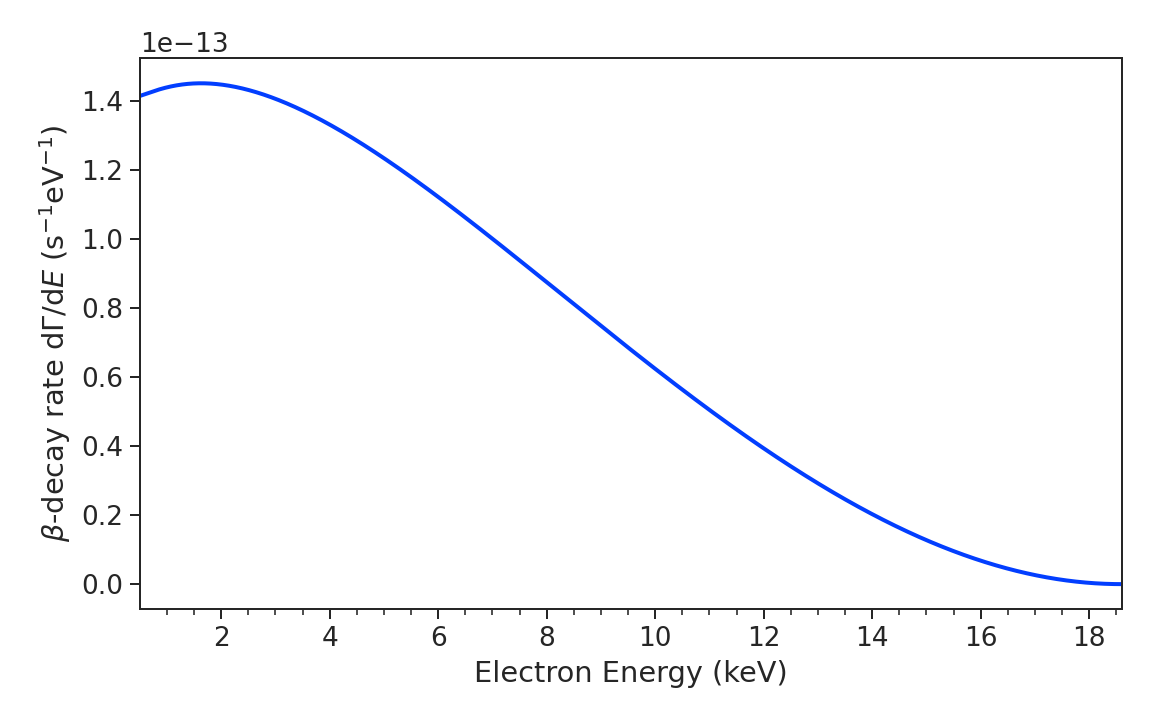
\includegraphics[width=0.7\textwidth]{figs/Chapter-2/230302_atomic_tritium_spectrum.png}
%    \caption{Caption}
%    \label{fig:chap2-tritium-spectrum}
%\end{figure}
where $G_F$ is the Fermi coupling constant, $V_{ud}$ is an element of the CKM matrix, $E$ is the kinetic energy of the electron, $\beta$ is the velocity of the electron divided by the speed of light, $E_0$ is the endpoint energy assuming zero neutrino mass, $F(Z,\beta)$ is the Fermi function, and $\Theta(E_0-E-m_i)$ is the Heaviside function, which enforces energy conservation. One can see that the decay spectrum is actually a combination of three spectra with different endpoints based on the values of the neutrino mass eigenstates, $m_i$. This produces "kinks" in the spectrum shape due to overlapping spectra with different endpoint values, but such an effect would be nearly impossible to resolve given the finite energy resolution of a real experiment. 

\begin{figure}[htbp]
    \centering
    \begin{subfigure}{0.6\textwidth}
        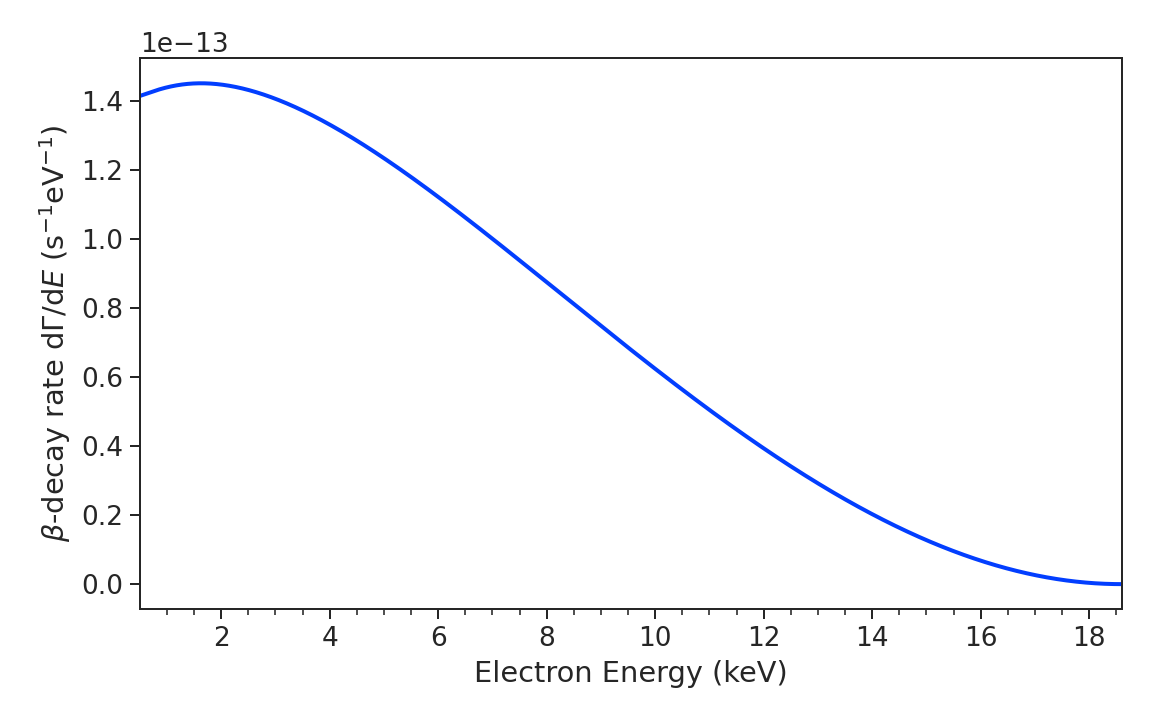
\includegraphics[width=\textwidth]{figs/Chapter-2/230302_atomic_tritium_spectrum.png}
        \caption{}
    \end{subfigure}
    \begin{subfigure}{0.6\textwidth}
        \includegraphics*[width=\textwidth]{figs/Chapter-2/230302_atomic_tritium_spectrum_near_endpoint.png}
        \caption{}
    \end{subfigure}
    \caption{The tritium beta-decay spectrum. The effect of a massive neutrino on the spectrum is to change its shape near the endpoint by an amount proportional to the size of the neutrino mass. A sufficiently high-statistic and high-resolution measurement of the spectrum endpoint would be able to measure the neutrino mass.}
    \label{fig:chap2-atomic-tritium-endpoint}
\end{figure}

The neutrino mass scale variable measured by beta-decay is given by 
\begin{equation}
    m_\beta^2=\sum_i{|U_{ei}|^2}m_i^2,
\end{equation}
where $m_\beta$ is the electron-weighted neutrino mass or simply "neutrino mass" for brevity. The quantity $m_\beta$ corresponds to a particular weighted sum of the neutrino masses, which is distinct from effective neutrino masses such as $m_{\beta\beta}$ \cite{FORMAGGIO20211}. Assuming unitarity, the neutrino mass can be expressed in terms of the PMNS matrix elements, squared mass differences, and the lightest neutrino mass eigenstate. For the normal mass ordering the equation is
\begin{equation}
    m_\beta^2=m^2_\textrm{least} + |U_{e2}|^2\Delta m_{21}^2 +|U_{e3}|^2\Delta m_{31}^2,
\end{equation} 
and for the inverted ordering the equation is 
\begin{equation}
    m_\beta^2=m^2_\textrm{least}+|U_{e1}|^2(-\Delta m_{32}^2-\Delta m_{21}^2)+|U_{e2}|^2(-\Delta m_{32}^2).
\end{equation}
Therefore, a measurement of the neutrino mass in combination with neutrino mixing parameters is effectively a measurement of $m_\textrm{least}$.

Since the neutrino mass is small ($<1$~eV), its effect on the spectrum is limited to the endpoint region. The affect of a non-zero neutrino mass on the endpoint spectrum is plotted for the reader in Figure \ref{fig:chap2-atomic-tritium-endpoint}. Resolving the small changes in the spectrum shape requires an experimental technique with high statistics, excellent energy resolution, and low background activity. 

%The KATRIN collaboration, utilizing a large MAC-E (magnetic adiabatic collimation with electrostactic) filter spectrometer recently obtained the best direct measurement of the neutrino mass, with a 90\% confidence upper limit of 0.8~eV. With more statistics the KATRIN collaboration estimates an ultimate sensitivity to neutrino masses of 0.2~eV.